\documentclass{article}
\usepackage[margin=0.6in]{geometry}
\usepackage{plex-sans}
\usepackage{enumitem}
\usepackage{float}
\usepackage{chngcntr}
\counterwithin{table}{section}
\usepackage{tikz}
\usepackage{longtable}

\title{SCADS System and Software Design Description}
\author{jake baldwin}
\date{\today}

\begin{document}
    \maketitle

    \section{Document Overview}\label{sec:document-overview}

        \subsection{Purpose}\label{ssec:purpose}

        The SCADS System and Software Design Description (SSDD) is the document
        specifying the system design and implementation decisions. The system
        strives to meet the requirements specified in the Software Requirements
        Specification (SRS). This compendium provides both high level system
        design and low level detailed implementation details.

        \subsection{Scope}\label{ssec:scope}

        This document covers the high level design and low level implementation
        details of such system to meet the requirements specified in the SRS,
        and the high level testing architecture. The full testing plan
        is specified in the Software Test Plan and Procedures (STPP) document,
        which is where the tests to verify the SRS requirements explicitly will
        live.

        \subsection{Related Documents}\label{ssec:related-documents}
            \begin{itemize}[label={}]
                \item The Software Development Plan (SDP)
                \item The Software Requirements Specification (SRS)
                \item The Software Test Plan and Processing Procedures (STP)
            \end{itemize}
        \subsection{Definitions and Acronyms}\label{ssec:definitions}

        The table below contains definitions and acronyms used within the 
        document.

        \begin{table}[H]
            \caption{Definitions and Acronyms}
            \vspace{4pt}
            \centering
            \renewcommand{\arraystretch}{1.4}
            \begin{tabular}{|l|p{14cm}|}
                \hline
                \textbf{Term} & \textbf{Definition} \\ \hline
                SCADS & Spacecraft Control Attitude Determination System \\ \hline
                SDP & Software Development Plan \\ \hline
                SSDD & System and Software Design Description \\ \hline
                STPP & Software Test Plan and Procedures \\ \hline
                TBD & To be determined \\ \hline
                FreeRTOS & Free Real-Time Operating System \\ \hline
            \end{tabular}
        \end{table}

    \section{Design Considerations}\label{sec:design-considerations}

        \subsection{Assumptions}\label{ssec:assumptions}

        \subsection{Constraints}\label{ssec:constraints}

        \subsection{Design Philosophy}\label{ssec:design-philosophy}

        \subsection{Key Trade Offs}\label{ssec:key-trades}

    \section{Overall System Architecture}\label{sec:overall-system-architecture}

        \subsection{System Architecture Overview}\label{ssec:system-architecture}

        The following figure contains the overall system architecture.

        \begin{figure}[H] 
            \centering
            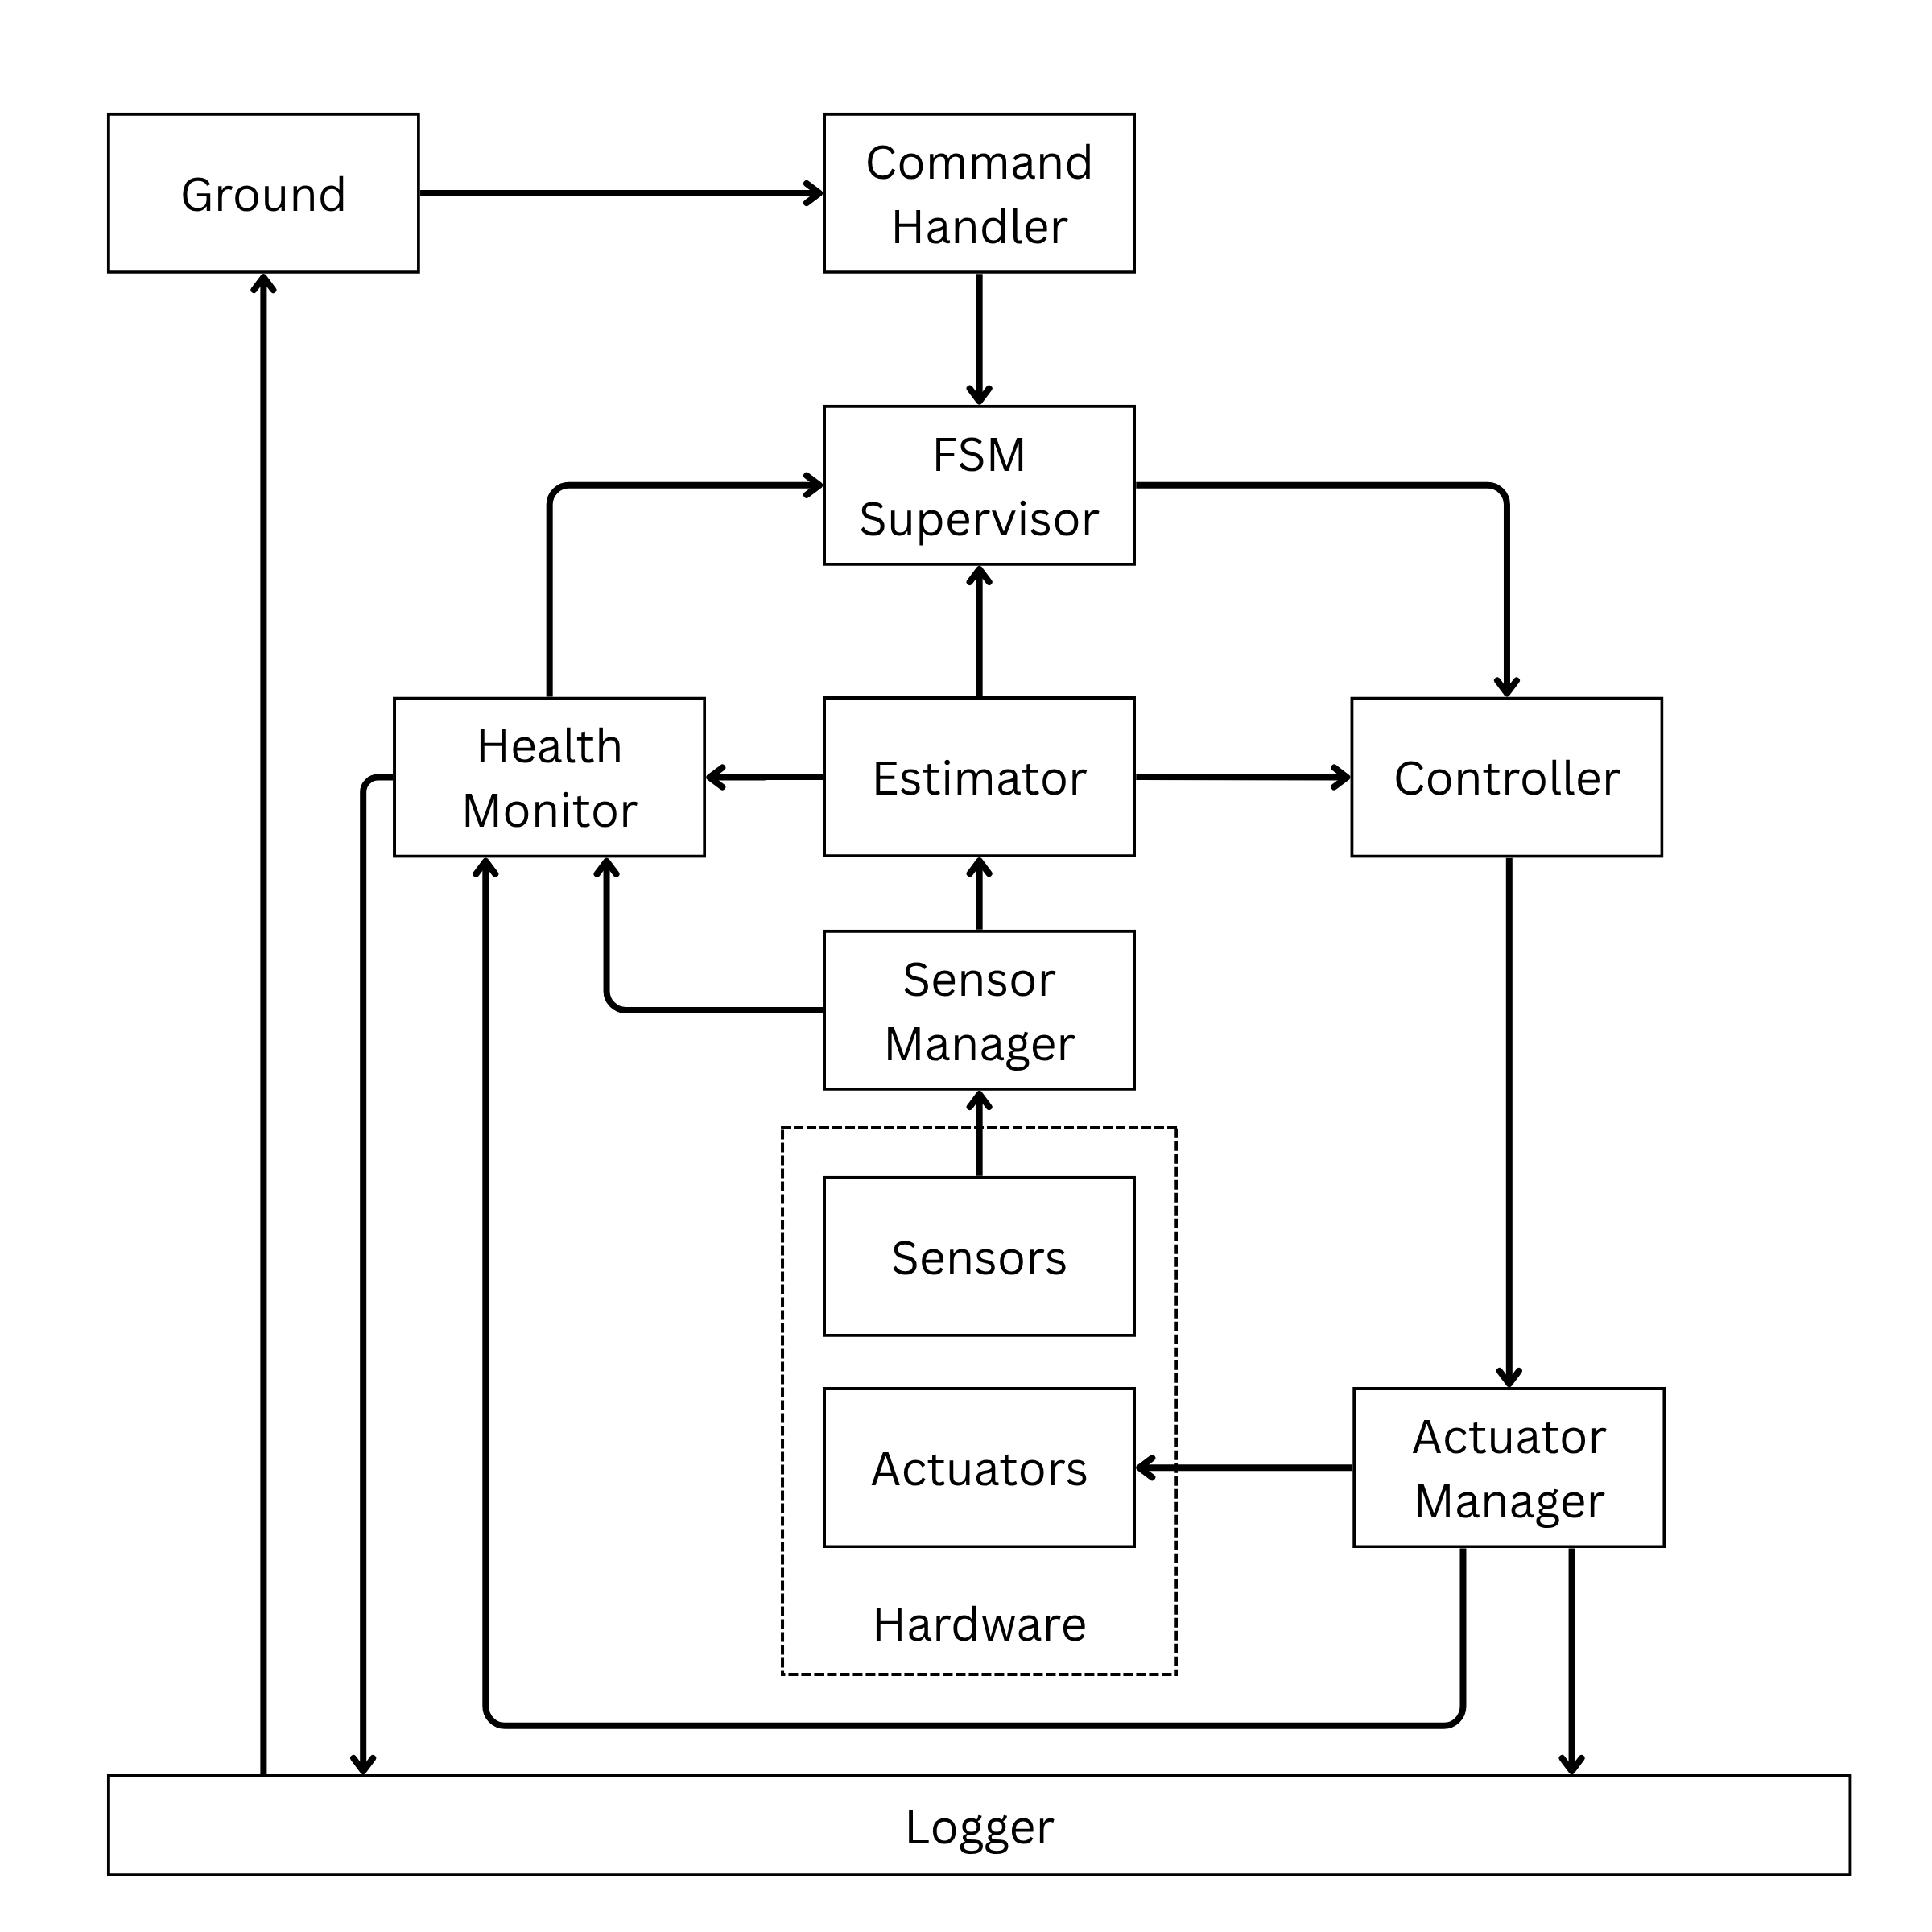
\includegraphics[width=0.9\textwidth]{../figures/scads-architecture.png}
            \caption{SCADS System Architecture}
            \label{fig:scads-architecture}
        \end{figure}

        \subsection{Hardware Platform}\label{ssec:hardware-platform}

        \subsection{FreeRTOS Task Structure}\label{ssec:freertos-task-structure}

        \subsection{Module Structure}\label{ssec:module-structure}

        \subsection{Data Flow}\label{ssec:data-flow}

    \section{Detailed Design}\label{sec:detailed-design}

        \subsection{Finite State Machine Implementation}\label{ssec:fsm}

        \subsection{Attitude Estimation}\label{ssec:attitude-estimation}

        \subsection{Attitude Control}\label{ssec:attitude-control}

            \subsubsection{Detumble Control}\label{sssec:detumble-control}

            \subsubsection{Safe Control}\label{sssec:safe-control}

            \subsubsection{Nominal Hold Control}\label{sssec:nominal-hold-control}

        \subsection{Sensor Data Acquisition}\label{ssec:sensor-acquisition}

        \subsection{Actuator Command Generation}\label{ssec:actuator-generation}

        \subsection{Health Monitoring}\label{ssec:health-monitoring}

        \subsection{Time Management}\label{ssec:time-management}

        \subsection{Fault Detection}\label{ssec:fault-detection}

    \section{Interface Design}\label{sec:interface-design}

        \subsection{Ground Command Interface}\label{ssec:ground-command-interface}

        \subsection{Telemetry Output Interface}\label{ssec:telemetry-interface}

        \subsection{Sensor Acquisition Interface}\label{ssec:sensor-interface}

        \subsection{Actuator Command Interface}\label{ssec:actuator-interface}

        \subsection{Inter-Task Communication}\label{ssec:inter-task-comm}

    \section{Memory and Resource Allocation}\label{sec:memory-layout}

        \subsection{Memory Layout}\label{ssec:memory-layout}

        \subsection{Stack Sizing}\label{ssec:stack-sizing}

        \subsection{CPU Budget}\label{ssec:cpu-budget}

    \section{Build and Deployment}\label{sec:build-and-deployment}

    \section{Test Architecture}\label{sec:test-architecture}

\end{document}

